\section{Results}

%How can I assess the quality of my Results section? To make a self-assessment of your Results section, you can ask yourself the following questions.
%    * Have I expressed myself as clear as possible, so the contribution of my results give stands out for the referees and readers?
%    * Have I limited myself to only reporting the key result or trends each figure and table conveys, rather than reiterating each value?
%    * Have I avoided drawing conclusions? (this is only tr,ue when the Results is an independent section)
%    * Have I chosen the best format to present my data (e.g. figure or table)? Have I ensured there is no redundancy between the figures and tables?
%    * Have I ensured my tables of results are comprehensive in the sense that they do not exclusively include points wich prove my point?
%    * Have I mentioned only what my readers specifically need to know and what I will subsequently refer to in the Discussion?
%    * Have I mentioned any parts of my methodology (e.g. selection and sampling procedures) wich could have affected my results?
%    * Have I used tenses correctly? past simple for your findings (in the passive form), present simply (descriptions of established scientific fact)


In this section, the results of Mapping are presented, firstly, we show an overview of the selected papers and after the answers to research questions and their findings.

\subsection{Overview}

In this study we identified 26 papers that used Machine Learning techniques for code smell identification. They were published between 1999 to 2016 and they used experimentation as methodology. 65\% of the papers were published in conferences and the other 37\% were published in journal. Only 5 of publications were represented by more than one publication venue: Annual Conference on Genetic and Evolutionary Computation; International Conference on Software Engineering;Journal of Systems and Software; Expert Systems with Applications; Journal of Software: Evolution and Process. These publications represented almost half of the selected papers as shown in Table \ref{tab:papersByPublication}.

\begin{table}[hbt]
\centering
\caption{Papers by publication}
\label{tab:papersByPublication}
\begin{tabular}{ll}
\hline
Publication &                                               \# of studies\\ \hline
Annual Conference on Genetic and Evolutionary Computation &     3   \\
International Conference on Software Engineering &              3   \\
Journal of Systems and Software &                               3   \\
Expert Systems with Applications &                              2   \\
Journal of Software: Evolution and Process &                    2   \\
Others &                                                        13  \\ \hline
\end{tabular}
\end{table}

Through the Figure \ref{fig:papersByYear}  it's possible to see the trend of publication years. The Figure \ref{fig:papersByYear} shows a small interest of studies to identify code smell using Machine Learning techniques between 2002 at 2014, but big interest in 2015 at 2016. The number of research in last two years overcame the numbers of previous years.  Worth remember that code smell term were used by Kent Beck in the late 1990's and the research about code smell were focused in other techniques as metrics. Detection of code smells based in machine learning techniques have not been largely explored~\citep{Fontana2013}.
%arranjar uma justificativa melhor
%Não achei a observação nesses artigos  - Bruno
%Confirming the observation of previous studies~\citep{rasool2015review, fontana2016comparing} which shows a growing interest in Machine Learning techniques for code smell identification.
% Do Rasool se não me engano me baseei na Table II, mas do Fontana eu também não achei, posso ter interpretado algo errado ou mudado algo no caminho quando estava escrevendo

\begin{figure}[hbt] 
    \centering
	\caption{Papers by year}
	\label{fig:papersByYear}
	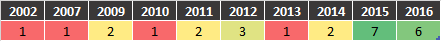
\includegraphics[]{imagens/papersByYear.png}
\end{figure}
%todos os papers usaram java? -Bruno
%23 ou 24 projetos de código fonte aberto
%os outros projetos que são 70% não nomearam os sistemas? % os dados do slr_protocol_results mostram mais de 65 projetos
All papers selected in this study identified code smells analyzing projects developed with Java language. From 26 papers, 23 used open source projects, while only 3 used private data source. We identified 88 open source projects as dataset used in research, the dataset more used was the Xerces, followed by JHotDraw, Eclipse Core and ArgoUML. Among the 88 datasets 62 of them were used only one time. As detailed by Table \ref{tab:opensourceTable}.

\begin{longtable}{||c|c||c||c|}
\caption{Used open source projects}
\label{tab:opensourceTable}
\\

\hline
	Software & Number of Papers & Software & Number of Papers \\ \hline
	Xerces & 6 & Apache Commons Logging & 1 \\ \hline
	JHotDraw & 5 & JDI-Ford & 1 \\ \hline
	Eclipse Core & 5 & Apache Derby & 1 \\ \hline
	ArgoUML & 4 & JFreeChart  & 1 \\ \hline
	JFreeChart & 3 & Apache James Mime4j & 1 \\ \hline
	GanttProject & 3 & JRDF & 1 \\ \hline
	Apache Cassandra & 2 & Apache Tomcat & 1 \\ \hline
	Rhino & 2 & Maven & 1 \\ \hline
	Qualitas Corpus & 2 & ApacheAnt & 1 \\ \hline
	GanttProject  & 2 & Pixelitor & 1 \\ \hline
	jEdit & 1 & ApacheAnt  & 1 \\ \hline
	Ant & 1 & sapphire & 1 \\ \hline
	Log4J  & 1 & Android API (framework-opt-telephony) & 1 \\ \hline
	And Engine & 1 & XWorks & 1 \\ \hline
	JabRef & 1 & BCEL & 1 \\ \hline
	Apache Commons Codec & 1 & Jboss & 1 \\ \hline
	Android API (tool-base) & 1 & Closure Compiler & 1 \\ \hline
	Apache Commons IO & 1 & JDK  & 1 \\ \hline
	nebula.widgets.nattable & 1 & dltk.core & 1 \\ \hline
	Apache Commons Lang & 1 & Android API (sdk) & 1 \\ \hline
	Xerces  & 1 & Android API (frameworks-base) & 1 \\ \hline
	JGraphx & 1 & Aardvark & 1 \\ \hline
	egit & 1 & platform.resources & 1 \\ \hline
	JHotDraw  & 1 & Gitblit & 1 \\ \hline
	FindBugs & 1 & Ant-Apache & 1 \\ \hline
	jUnit & 1 & Google Guava & 1 \\ \hline
	FreeMind  & 1 & ANTLR & 1 \\ \hline
	Lucene  & 1 & graphiti & 1 \\ \hline
	GanttAzureus & 1 & Xom & 1 \\ \hline
	Mongo DB & 1 & Guava & 1 \\ \hline
	Android API (frameworks-support) & 1 & Apache Ant & 1 \\ \hline
	Nutch  & 1 & Hibernate & 1 \\ \hline

\end{longtable}


\subsection{Which code smells are addressed when using Machine Learning techniques for the identification?}

In this study, we used the 22 code smells defined by~\cite{fowler1999refactoring} as base for our classification, we also used 3 of the anti-patterns defined by~\citep{brown1998antipatterns} related to code related design flaws. There is also the "others" classification meant to capture smells defined by other authors and code-flaws not related to a specific smell, since the authors aim at code metrics optimization instead of a specific smell.

%código duplicado ficou em outra classificação? - Bruno Zhang citou que código duplicado é mais estudo nos code smells. Mas a o mapeamento não mostrou isso
Comparing the studied code-related design flaws using machine learning, the ones with higher appearance were Feature Envy (FE) smell and BLOBs both studied by 5 papers, followed by Long Methods (LM) that appeared in 4. While Comments (COM), Primitive Obsession (PO), Refused Bequest, Alternative Classes with Different Interfaces (ACDI) and Incomplete Library Class (ILC) were not addressed by any of the studied papers. The distribution of the smells is show in Figure \ref{fig:papersBySmell}. Except for the duplicated code which is usually the mainly studied smell, the other smells are coherent with the ones identified by~\cite{zhang2011code} in his review. The others category, composed mainly by optimization in the code metrics appeared 8 times, using alternatives to the traditional code smells. %O que nós fizemos com estes outros?

\begin{figure}[!ht] 
    \centering
	\caption{Papers by Code Smell}
	\label{fig:papersBySmell}
	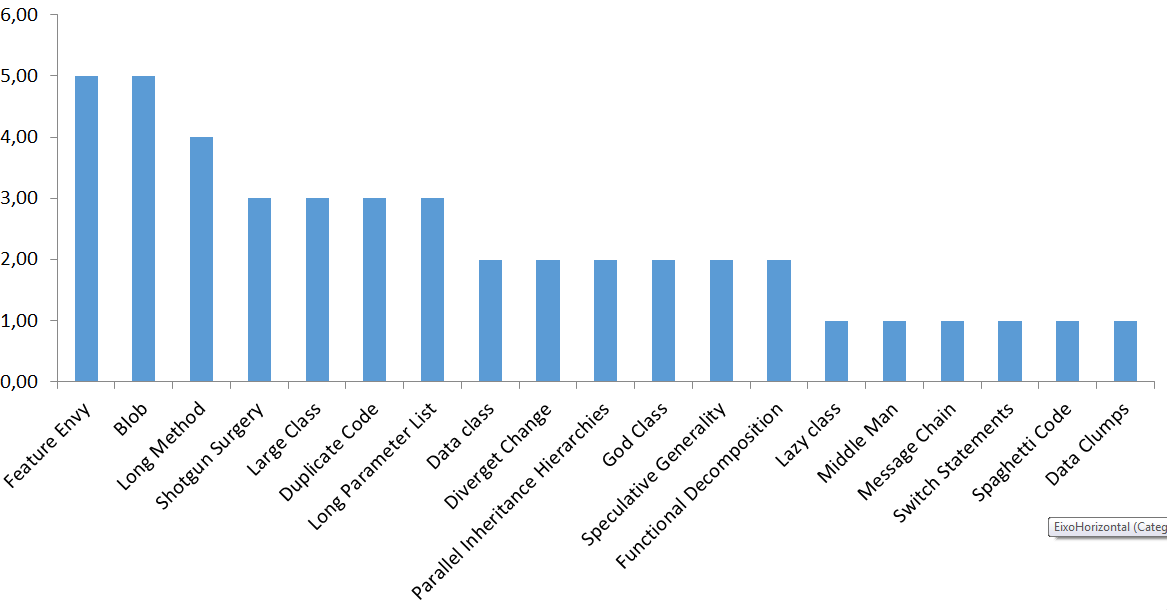
\includegraphics[width=0.95\textwidth]{imagens/papersBySmell.png}
\end{figure}

% Montar um gráfico que abrange as classificações dos tipos e dos bad smells - Decidir entre o o gráfico ou a frase abaixo. 
% Gerar um insight para falar do gráfico - Bruno
When grouping by the classification defined by~\cite{mantyla2003bad} it is possible to observe that the main focus regarding the addressed type of smell are the Bloaters representing 35\% of the studied smells. Follows to this: The Dispensables (15\%); The Object-Orientation Abusers (9\%); The Change Preventers (9\%); The Couplers (9\%); The Encapsulators (4\%). The other code smells, mainly represented by metrics-based representations, represent 17\%. As detailed on Figure \ref{fig:papersBySmellType}.

%alterar o gráfico para deixar mais nítido.

\begin{figure}[!ht] 
    \centering
	\caption{Papers by Code Smell Type}
	\label{fig:papersBySmellType}
	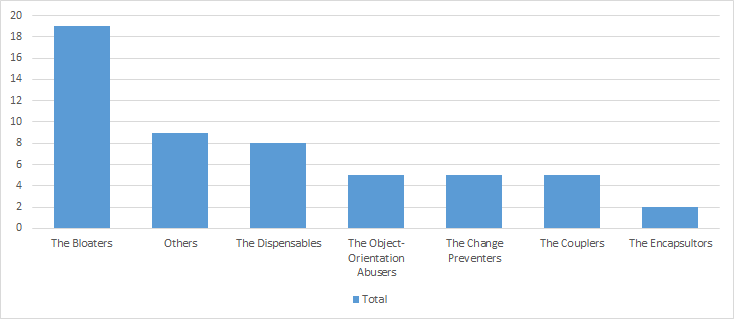
\includegraphics[width=0.95\textwidth]{imagens/papersBySmellType.png}
\end{figure}

%
%%There are a strongest co-ocorrece of code smells in studies. For instance, the research between...
% Não entedi porque eles são relacionados só pq foram definidos or brown? - Bruno
When studying the smells usually studied together, one of the strongest co-occurrence is between BLOB, Spaghetti Code (SC) and Functional Decomposition (FD), one of the main reasons is that they use the anti-patterns definition  by~\citet{brown1998antipatterns}, while the others are defined by ~\citet{fowler1999refactoring}. Duplicated code also had a strong co-occurrence with Divergent Changes (DCP) and Shotgun Surgery (SS), but the reciprocal was not true, one of the explanations is that Duplicated Code (DUC) is usually studied alone. Feature Envy also receives highlight when comparing smells usually studied together, it is studied together with part of the smells. Others that deserve mention are Long Parameter List (LPL), Long Methods (LM) and Large Class (LC). The co-occurrence matrix is shown in details in Figure \ref{fig:smellsCoOccurrence}.  %essa figura não disse o q está descrito no texto. Talvez um gráfo represente bem essa relação. Podemos tentar gerar no gephi mesmo

\begin{figure}[!ht] 
    \centering
	\caption{Graph representing which smells worked in the same paper}
	\label{fig:smellsCoOccurrence}
	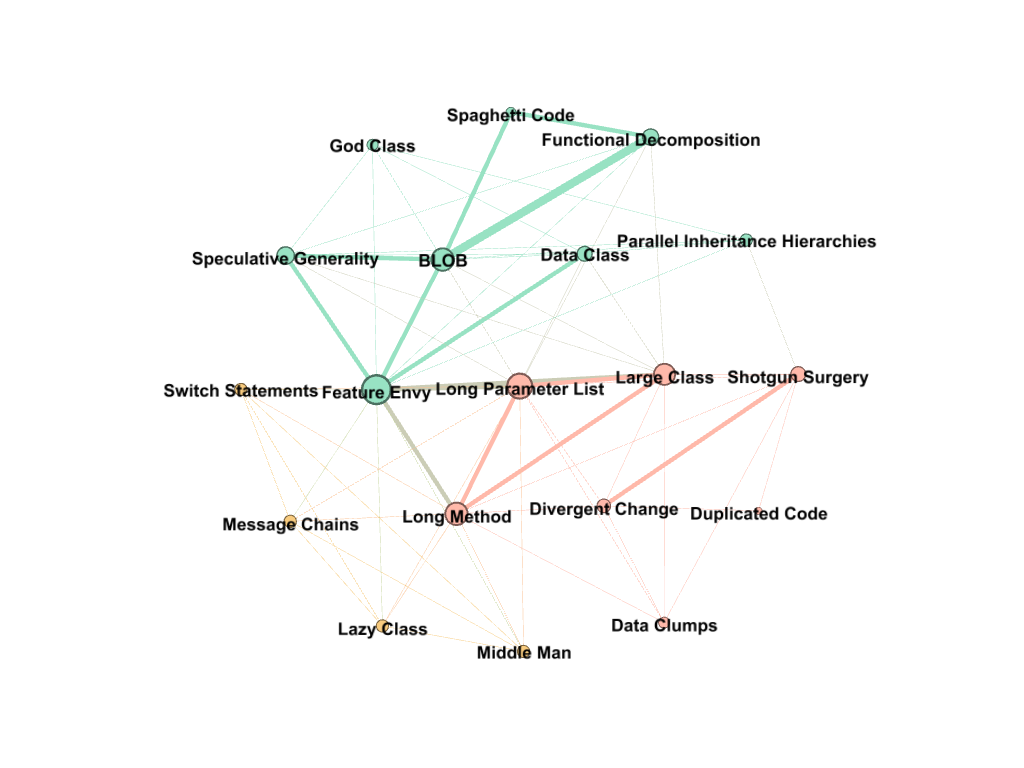
\includegraphics[width=0.95\textwidth]{imagens/smells_coocurrence_graph.png}
\end{figure}


\subsection{Which Machine Learning techniques are used when identifying code smells?}

The leading technique in the analyzed papers was the Genetic Algorithm which appeared 8 times, this technique is used mainly in search-based techniques, and focuses on optimizing one or more metric by mutating and evolving the code. Followed by Naive Bayes Classifiers that appeared 4 times. While a approaches such as: Linear discriminant analysis (LDA); Decision Tree; Support; Vector Machine (SVM); Directed Acyclic Graph (DAG); Text-Based - appeared only once. The distribution can be visualized in Figure \ref{fig:papersByMLTechnique}.

\begin{figure}[!ht] 
    \centering
	\caption{Papers by Machine Learning Technique}
	\label{fig:papersByMLTechnique}
	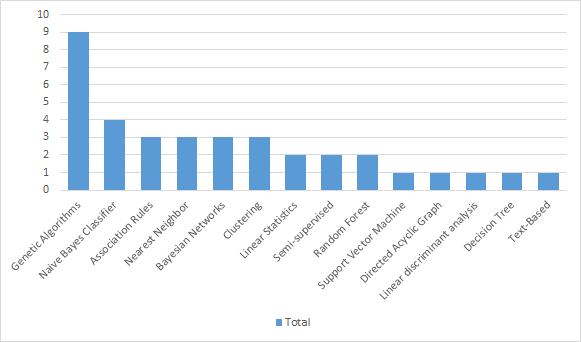
\includegraphics[width=0.95\textwidth]{imagens/papersByMLTechnique.png}
\end{figure}


Regarding the kind of technique used the supervised techniques were the main one, being used in 32 tests (88\%); Semi supervised and unsupervised techniques appeared only 2 (6\%) times which. The results was expected since supervised tests are the greatly used in researches~\citep{kotsiantis2007supervised}.

\subsection{Which Machine Learning techniques are most used for each kind of code smell?}

The smells addressed by the techniques were coherent with the smells that appeared in the related papers, showing a high level of redundancy. The smell focused by the majority of the techniques was Feature Envy (FE), which was aimed by 9 techniques (64\%). Followed by Long Method (LM) with 8 techniques (57\%) and Long Parameter List (LPL) with 7 (50\%). From the smells targeted by the studied papers, the ones covered by less techniques were Speculative Generality (SG), Spaghetti Code (SC), Data Class (DAC),  God Class (GC), Parallel Inheritance (PIH) and Divergent Changes (DCP) with 2 techniques each (14\%).

From a Machine Learning technique perspective, the Association Rules techniques was the technique with broader usage, covering 13 smells (59\% of them), followed by linear statistics with 11 smells (50\%), Naive Bayes and Random Forest with 9 smells (43\%). While Text-Based and Linear Discriminant Analysis with 1 smell (5\%) are in the lower half.


When comparing the number of times a code smell was addressed by a given technique, there was no clear relationship. Although the smells coverage is higher for a given technique, e. g., Feature Envy (FE) and Bayesian Network, it does not displays a clear pattern. The relation between smells and techniques can be visualized in Figure \ref{fig:smellsXMLTechniques}

\begin{figure}[!ht] 
    \centering
	\caption{Number of times a smell was studied with another by technique}
	\label{fig:smellsXMLTechniques}
	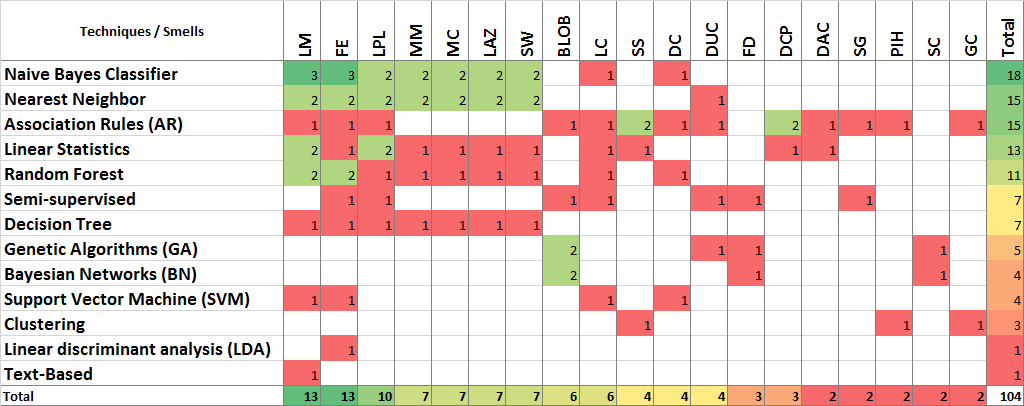
\includegraphics[width=0.95\textwidth]{imagens/smellsXMLTechniques.png}
\end{figure}

However when comparing the smells by type, we found out that the Association Rules technique with a relevant focus on the Change Preventers type of smell, as the graph nature of technique allows it to analyze the relationship between methods and classes. The other smell types followed the same patterns presented when comparing the coverage by papers and the classifiers the same pattern as discussed previously.

\begin{figure}[!ht] 
    \centering
	\caption{Code Smell type by Machine Learning technique}
	\label{fig:smellsTypeXMLTechniques}
	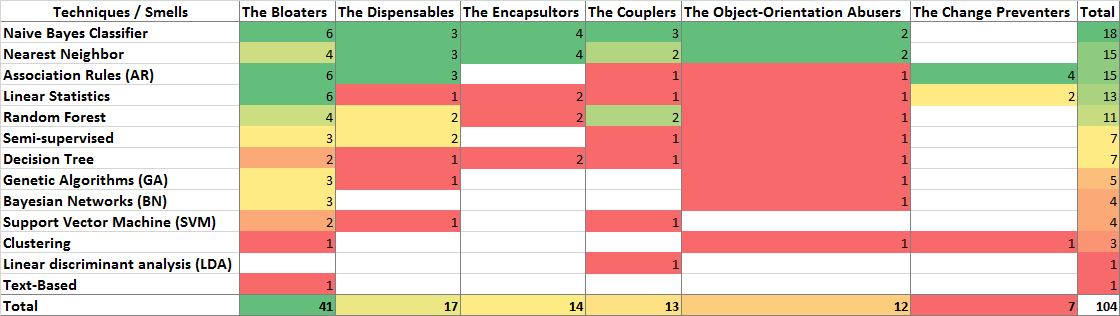
\includegraphics[width=0.95\textwidth]{imagens/smellsTypeXMLTechniques.png}
\end{figure}

\subsection{Which Machine Learning techniques performs better for each smell?}

One hardship we found when comparing the techniques performance is the lack of standardized data. 14 out of the 26 papers provided performance info. From those, 13 provided precision data, 12 provided recall values and only 6 provided us with F-measures, we used the recall and precision data provided by the other to calculate their f-measures as well to have a better comparison measure. To have comparable parameters we also selected only the papers that used the same baseline as the majority of the articles, in this case a manual annotation of the code smells.

In terms of f-measure the best average performance was provided by Decision Tree, followed by Random Forest, Semi-supervised and Nearest Neighbor techniques. While Text-Based, Linear Discriminant Analysis and Naive Bayes presented the worst performance overall between the studied practices, as demonstrated by Figure \ref{fig:fmeasureByTechniques}.

\begin{small}
\begin{longtable} {|l|l|l|l|l|}
\caption{F-Measure summary per smell and technique: Ordered by the max f-measure}
\label{tab:opensourceTable}
\\

\hline
Smell            & Technique                          & Min   & Median & Max    \\ \hline
MM - Middle Man              & Decision Tree          & 1.00  & 1.00   & 1.00  \\ \hline
MM - Middle Man              & Linear Statistics      & 0.85  & 0.85   & 0.85  \\ \hline
MM - Middle Man              & Nearest Neighbor       & 0.85  & 0.85   & 0.85  \\ \hline
MM - Middle Man              & Random Forest          & 0.71  & 0.71   & 0.71  \\ \hline
MM - Middle Man              & Naive Bayes Classifier & 0.14  & 0.38   & 0.62  \\ \hline\hline

SG - Speculative Generality  & Association Rules (AR) & 0.86  & 1.00   & 1.00  \\ \hline\hline

DCP - Divergent Change       & Association Rules (AR) & 0.55  & 0.85   & 1.00  \\ \hline\hline

LM - Long Method             & Association Rules (AR) & 0.99  & 0.99   & 0.99  \\ \hline
LM - Long Method             & Random Forest          & 0.86  & 0.92   & 0.99  \\ \hline
LM - Long Method             & Decision Tree          & 0.86  & 0.92   & 0.98  \\ \hline
LM - Long Method             & Support Vector Machine & 0.69  & 0.83   & 0.97  \\ \hline
LM - Long Method             & Naive Bayes Classifier & 0.54  & 0.60   & 0.93  \\ \hline
LM - Long Method             & Nearest Neighbor       & 0.89  & 0.90   & 0.90  \\ \hline
LM - Long Method             & Linear Statistics      & 0.84  & 0.84   & 0.84  \\ \hline
LM - Long Method             & Text-Based             & 0.56  & 0.62   & 0.71  \\ \hline\hline

LC - Large Class             & Random Forest          & 0.97  & 0.97   & 0.97  \\ \hline
LC - Large Class             & Association Rules (AR) & 0.97  & 0.97   & 0.97  \\ \hline
LC - Large Class             & Decision Tree          & 0.96  & 0.96   & 0.96  \\ \hline
LC - Large Class             & Naive Bayes Classifier & 0.96  & 0.96   & 0.96  \\ \hline
LC - Large Class             & Support Vector Machine & 0.73  & 0.85   & 0.96  \\ \hline\hline

LPL - Long Parameter List    & Random Forest          & 0.97  & 0.97   & 0.97  \\ \hline
LPL - Long Parameter List    & Linear Statistics      & 0.95  & 0.95   & 0.95  \\ \hline
LPL - Long Parameter List    & Nearest Neighbor       & 0.92  & 0.92   & 0.92  \\ \hline
LPL - Long Parameter List    & Decision Tree          & 0.92  & 0.92   & 0.92  \\ \hline
LPL - Long Parameter List    & Naive Bayes Classifier & 0.31  & 0.32   & 0.33  \\ \hline\hline

SS - Shotgun Surgery         & Decision Tree          & 0.97  & 0.97   & 0.97  \\ \hline
SS - Shotgun Surgery         & Nearest Neighbor       & 0.89  & 0.90   & 0.91  \\ \hline
SS - Shotgun Surgery         & Linear Statistics      & 0.89  & 0.89   & 0.89  \\ \hline
SS - Shotgun Surgery         & Random Forest          & 0.89  & 0.89   & 0.89  \\ \hline
SS - Shotgun Surgery         & Naive Bayes Classifier & 0.52  & 0.61   & 0.70  \\ \hline\hline

FE - Feature Envy            & Decision Tree          & 0.96  & 0.96   & 0.96  \\ \hline
FE - Feature Envy            & Support Vector Machine & 0.69  & 0.83   & 0.96  \\ \hline
FE - Feature Envy            & Naive Bayes Classifier & 0.24  & 0.26   & 0.95  \\ \hline
FE - Feature Envy            & Random Forest          & 0.94  & 0.94   & 0.94  \\ \hline
FE - Feature Envy            & Association Rules (AR) & 0.86  & 0.86   & 0.86  \\ \hline
FE - Feature Envy            & Nearest Neighbor       & 0.84  & 0.84   & 0.84  \\ \hline
FE - Feature Envy            & Linear Statistics      & 0.75  & 0.75   & 0.75  \\ \hline\hline

DUC - Duplicated Code        & Semi-supervised        & 0.96  & 0.96   & 0.96  \\ \hline
DUC - Duplicated Code        & Association Rules (AR) & 0.72  & 0.85   & 0.85  \\ \hline\hline

MC - Message Chains          & Linear Statistics      & 0.86  & 0.86   & 0.86  \\ \hline
MC - Message Chains          & Nearest Neighbor       & 0.86  & 0.86   & 0.86  \\ \hline
MC - Message Chains          & Random Forest          & 0.80  & 0.80   & 0.80  \\ \hline
MC - Message Chains          & Naive Bayes Classifier & 0.67  & 0.71   & 0.76  \\ \hline
MC - Message Chains          & Decision Tree          & 0.66  & 0.66   & 0.66  \\ \hline\hline

GC - God Class               & Clustering             & 0.66  & 0.72   & 0.82  \\ \hline\hline

BLOB                         & Bayesian Networks (BN) & 0.60  & 0.69   & 0.79  \\ \hline\hline
\end{longtable}

\end{small}

\begin{figure}[!ht] 
    \centering
	\caption{Machine Learning techniques F-measure Box-plot}
	\label{fig:fmeasureByTechniques}
	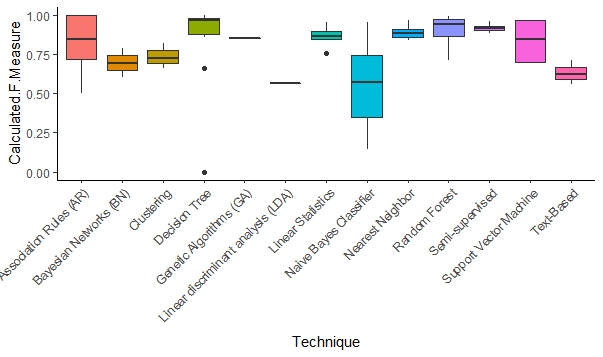
\includegraphics[width=0.9\textwidth]{imagens/fmeasureByTechniques.png}
\end{figure}

When comparing the results by f-measure as demonstrated by Figure \ref{fig:techniqueXSmellFMeasure}, it is possible to notice that the Association Rules technique performed above the others for Divergent Changes (DCP) and Speculative Generality (SG) smells, the ones covered by only this technique. But performs poorly for Duplicated Code (DUC) and Feature Envy (FE), when compared to the other techniques. Decision tree was also the best performing technique for Middle Man and Shotgun Surgery smells, while Random Forest had an outstanding performance for Long parameter list and Semi-Supervised techniques for Duplicated Code. Naive Bayes on the other side, performed poorly for Long Parameter List, Middle Man and Shotgun Surgery. In regard to the other smells, there was no outstanding technique.

\begin{figure}[!ht] 
    \centering
	\caption{Technique F-Measure by code smell}
	\label{fig:techniqueXSmellFMeasure}
	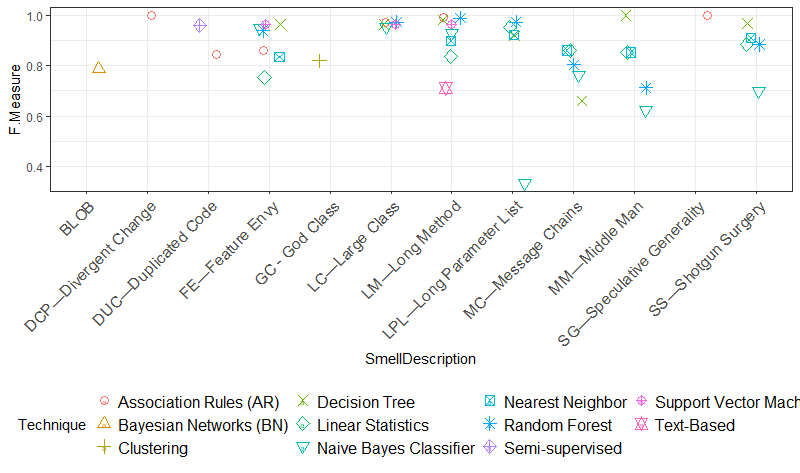
\includegraphics[width=0.95\textwidth]{imagens/TechniqueXSmellFMeasure.png}
\end{figure}

When analyzing the techniques by precision, the Linear Discriminant Analysis technique presented the best average performance, followed respectively to its performance by Association Rules, Semi-supervised and Decision Tree. In this aspect the worst performing techniques were the Bayes based techniques: Naive Bayes Classifier and Bayesian Networks. The results can be visualized in Figure \ref{fig:precisionByTechniques}.

\begin{figure}[!ht] 
    \centering
	\caption{Machine Learning techniques Precision Box-plot}
	\label{fig:precisionByTechniques}
	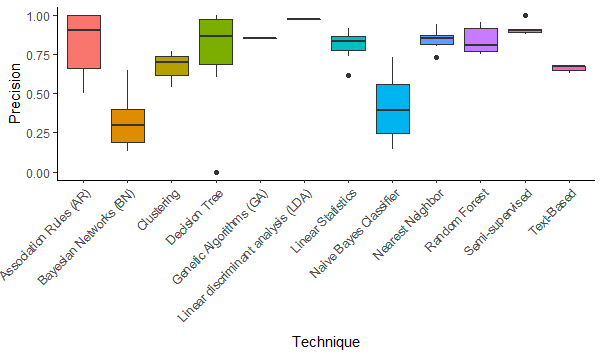
\includegraphics[width=0.9\textwidth]{imagens/precisionByTechniques.png}
\end{figure}

Comparing the techniques by precision, Association Rules, also demonstrated an outstanding performance on Divergent Changes (DCP) and Speculative Generality (SG), where it is the only technique used. Semi-supervised techniques had an outstanding performance for Duplicated Code (DUC), Random Forest for FE and Decision Tree for Lazy Class (LZC) and Middle Man (MM) also deserves mention. We had the Bayesian Networks and Naive Bayes Classifiers performing poorly than the other techniques on the smells. Those observations are displayed in Figure \ref{fig:techniqueXSmellPrecision}.

\begin{figure}[!ht] 
    \centering
	\caption{Technique Precision by code smell}
	\label{fig:techniqueXSmellPrecision}
	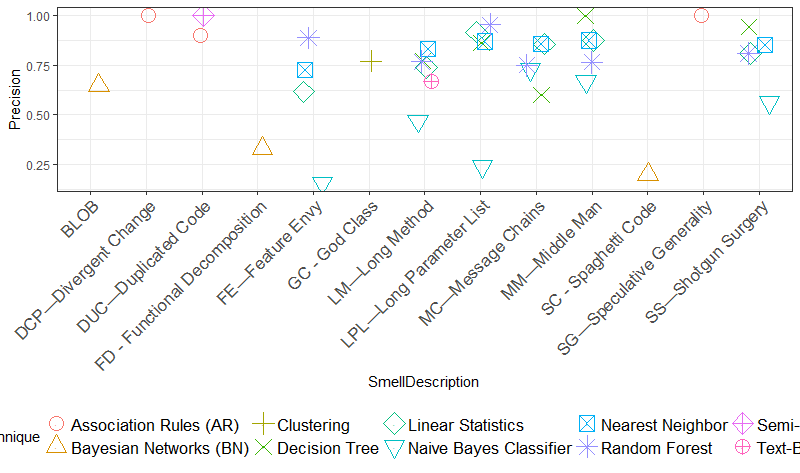
\includegraphics[width=0.95\textwidth]{imagens/TechniqueXSmellPrecision.png}
\end{figure}

When compared by recall, the techniques, in general, performed above 80\%. The best performing techniques under this perspectives were: Bayesian Networks, Decision Tree, Random Forest, Nearest Neighbor, Linear statistics, Semi-supervised, Genetic Algorithm and Clustering. While the worst performing was Naive Bayes classifier, Text-Based and Linear Discriminant Analysis, as displayed by Figure \ref{fig:recallByTechnique}.

\begin{figure}[!ht] 
    \centering
	\caption{Machine Learning techniques recall Box-plot}
	\label{fig:recallByTechnique}
	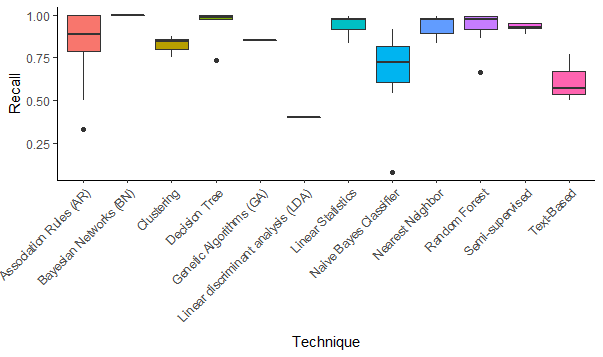
\includegraphics[width=0.9\textwidth]{imagens/recallByTechnique.png}
\end{figure}

%Calcular o F-measure de todos os papers para comparar - Bruno
Assessing the technique by smells under a Recall perspective as demonstrated in Figure \ref{fig:techniqueXSmellRecall}. As occurred in the previous perspective we have the Naive Bayes classifier performing worst in general, other techniques which displayed a bad performance was Random Forest for Middle Man (MM), Decision Tree for Message Chain (MC) and Text-Based technique for Long Method (LM).

\begin{figure}[!ht] 
    \centering
	\caption{Technique Recall by code smell}
	\label{fig:techniqueXSmellRecall}
	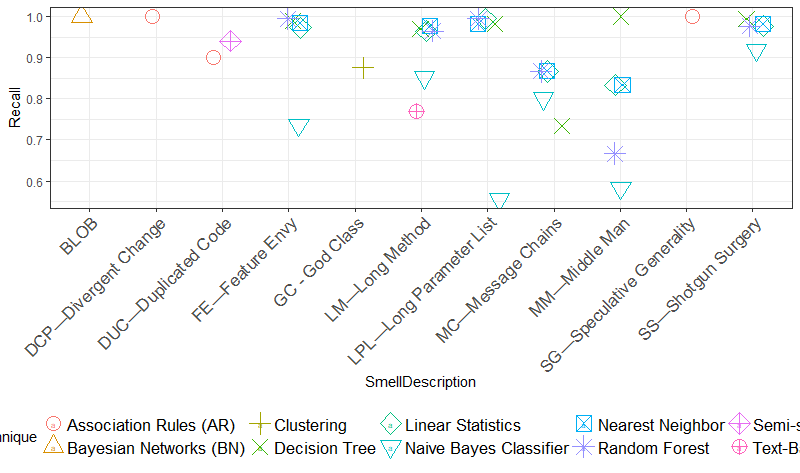
\includegraphics[width=0.95\textwidth]{imagens/TechniqueXSmellRecall.png}
\end{figure}

%as bases de dados podem ter influenciado no resultado? Seria interessante mostrar as técnicas seperadas por base dados. tipo - Usando Jhot eles procuraram os code smells x com tecnica y -Bruno

%montar uma analise de qual dataset foi utilizado para detectar qual code smell e com qual técnica de ML - Bruno
% ideia verificar o tratamento dos dados. Se ele teve que transformar os dados para um xml, csv, grafo, uml etc...
%%%%%%%%%
\section{Discussion}
\label{sec:discussion}
%%%%%%%%%

This studied tried to comprehend the patterns regarding machine learning applied for code smells identification. The study covered the papers in the period of 1999 to 2016, however no paper was published on the matter for about 2 years after the publication of the code smells by~\cite{fowler1999refactoring}, and it has only been an active topic research for the last 2 years, as shown on Table \ref{tab:papersByPublication}.

Studying the smells it was possible to assert that contrary to other studies~\citep{fowler1999refactoring, rasool2015review, fernandes2016review} that showed the Duplicated Code as the leading  smell, the ones using Machine Learning showed more concern about Feature Envy, BLOB and Long Methods, focusing heavier on non-structural smells. There is also a increasingly focus on metrics aimed technique, that seek the improvement of code metrics instead of aiming at a specific smell.

Regarding the techniques, although techniques such as Naive Bayes and Nearest Neighbor have been used more frequently than the others due to their simplicity, on the overall we did not find any killer technique receiving more attention, corroborating with the study by~\cite{fernandes2016review}, which found a high redundancy between the detected smells. The exception was the Association Rules, which outperformed the others when used for Change Preventers smells. We can also conclude, from the gathered data, the flexibility of the Machine Learning techniques, given the heterogeneous nature of the researched smells.

Comparing the performances we found that in average Decision Tree, followed by Random Forest, Semi-supervised and Nearest Neighbor classifiers outperformed the other techniques, while Text-Based, Linear Discriminant Analysis and Naive Bayes presented the worst performance overall between the studied practices, going against~\cite{fontana2016comparing} findings that found the Bayes approaches performing better for different code smells. There were also techniques that performed better for specific smells such as Association Rules for Divergent Changes and Speculative Generality, Decision tree for Lazy class, Middle Man and Shotgun Surgery smells, Random Forest for Long parameter list and Semi-Supervised techniques for Duplicated Code. 

This study also found that the papers lack comparable results, using the same data and performance metrics, a recurring problem in a significant number of studies so far~\citep{rattan2013software, al2015identifying, rasool2015review, fernandes2016review}. This factors turns the comparison of performance metrics between techniques a harder and inaccurate task, making the results less reliable and the studies harder to reproduce.
